\chapter{Обобщенная модель Изинга на квадратной решетке при учете декорирования}\label{ch:ch6}


\section{Точное решение обобщенной модели Изинга на квадратной решетке с учетом декорирования}

 \begin{figure}[h]
	\center{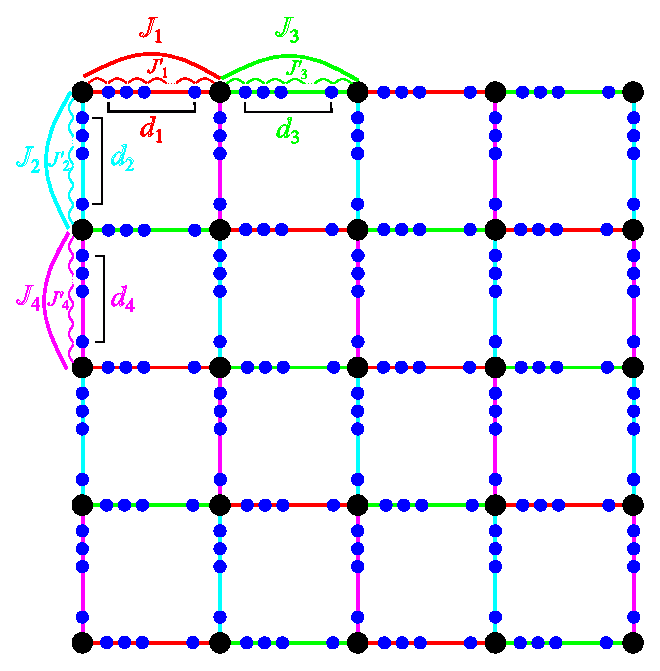
\includegraphics[width=0.55\linewidth]{part6/genDecorLattice.eps}}
	\caption{Квадратная решетка с двумя трансляциями при учете декорирования}
	\label{squareDecor}
\end{figure}

\section{Спонтанная намагниченность обобщенной модели Изинга на квадратной решетке с учетом декорирования}



\section{Термодинамические, фрустрационные особенности обобщенной модели Изинга на квадратной решетке при учете декорирования}

 \begin{figure}[h]
	\begin{minipage}{0.47\linewidth}
		\center{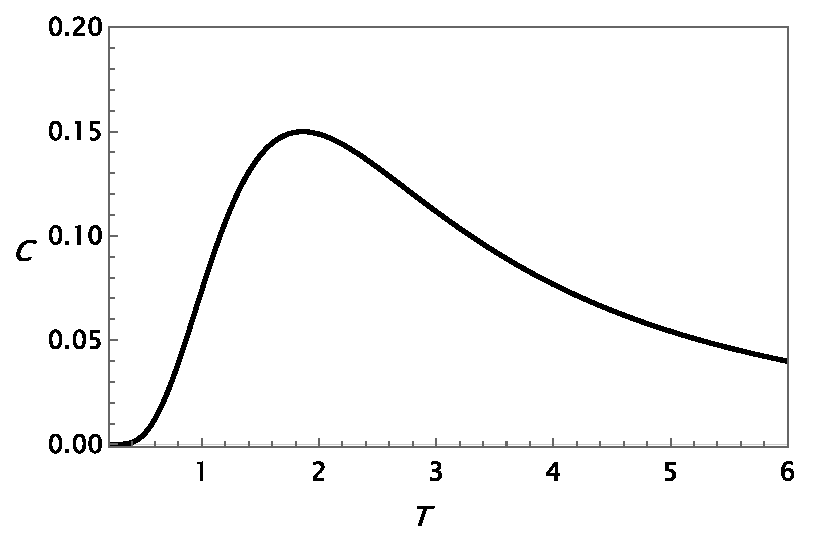
\includegraphics[width=1\linewidth]{part6/0transCap.eps} \\ а)}
	\end{minipage}
	\hfill
	\begin{minipage}{0.47\linewidth}
		\center{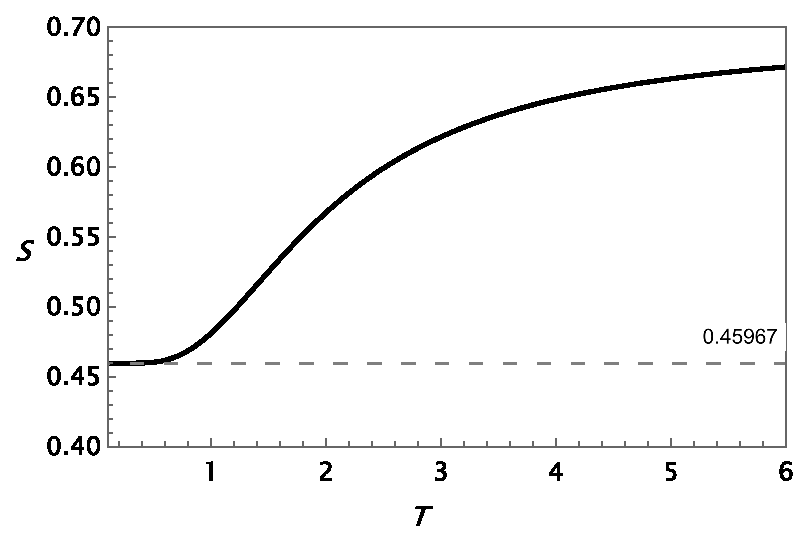
\includegraphics[width=1\linewidth]{part6/0transEnt.eps} \\ б)}
	\end{minipage}
	\caption{$J_1 = -1, J_2 = -1, J_3 = -1, J_4 = -1, J_{d_1} = 1, J_{d_2} = 1, J_{d_3} = 1, J_{d_4} = 1$ и $d_1 = 2, d_2 = 2, d_3 = 1, d_4 = 1$}
	\label{0trans}
\end{figure}

 \begin{figure}[h]
	\begin{minipage}{0.47\linewidth}
		\center{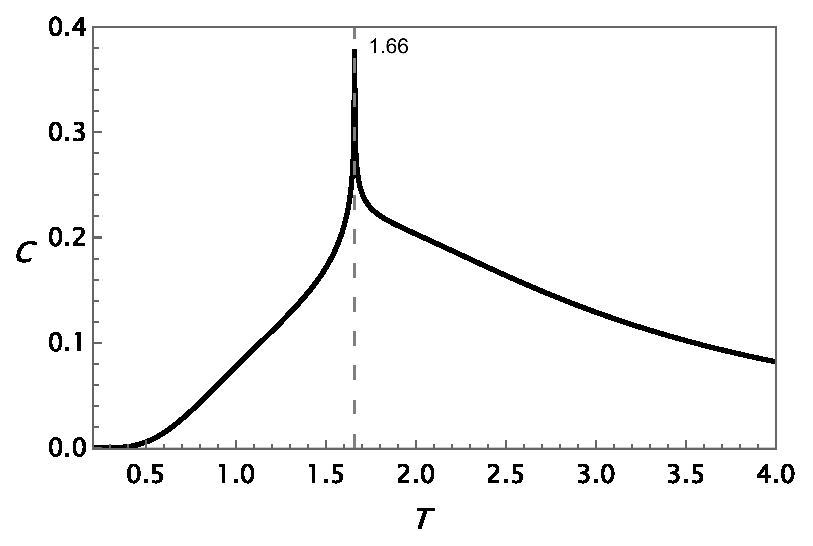
\includegraphics[width=1\linewidth]{part6/1transCap.eps} \\ а)}
	\end{minipage}
	\hfill
	\begin{minipage}{0.47\linewidth}
		\center{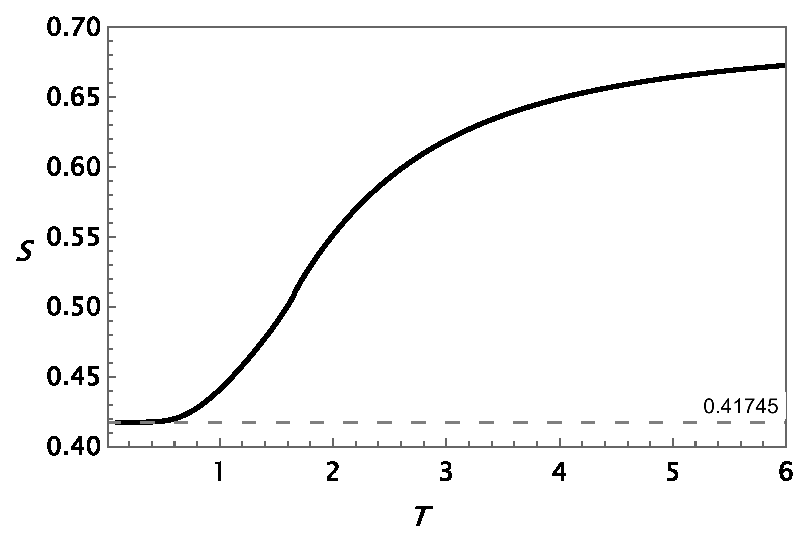
\includegraphics[width=1\linewidth]{part6/1transEnt.eps} \\ б)}
	\end{minipage}
	\vfill
	\begin{minipage}{0.47\linewidth}
		\center{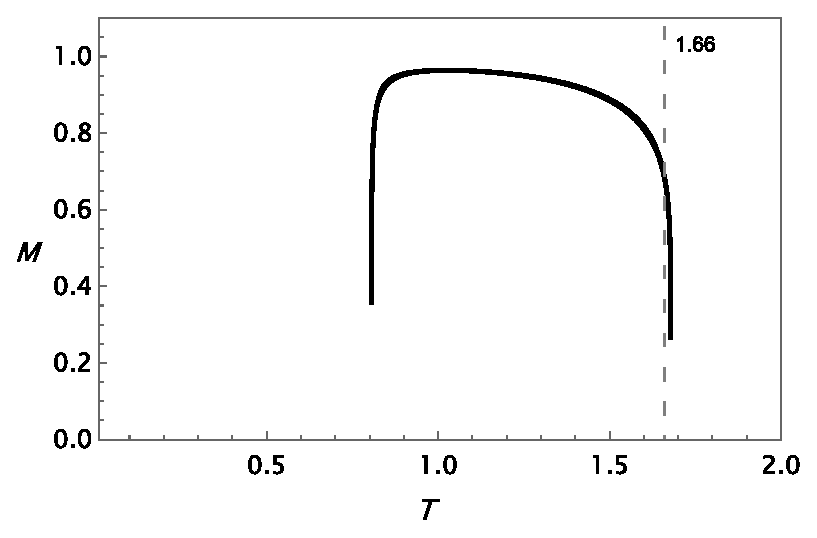
\includegraphics[width=1\linewidth]{part6/1transMag.eps} \\ б)}
	\end{minipage}
	\caption{$J_1 = -1, J_2 = -1, J_3 = -1, J_4 = -1, J_{d_1} = 1, J_{d_2} = 1, J_{d_3} = 1, J_{d_4} = 1$ и $d_1 = 2, d_2 = 3, d_3 = 1, d_4 = 3$}
	\label{1trans}
\end{figure}

 \begin{figure}[h]
	\begin{minipage}{0.47\linewidth}
		\center{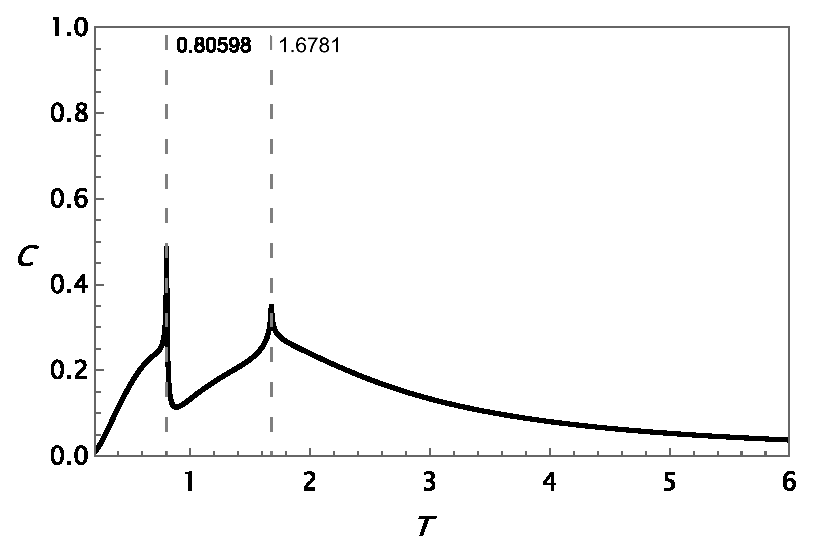
\includegraphics[width=1\linewidth]{part6/2transCap2.eps} \\ а)}
	\end{minipage}
	\hfill
	\begin{minipage}{0.47\linewidth}
		\center{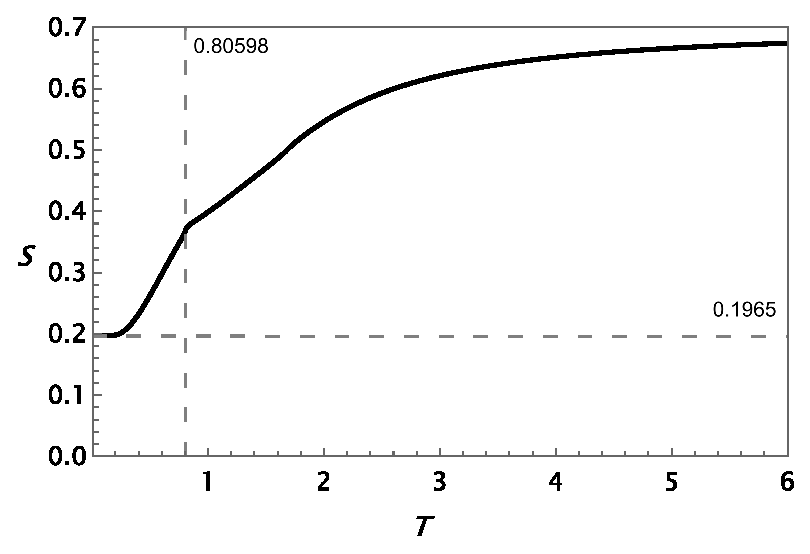
\includegraphics[width=1\linewidth]{part6/2transEnt2.eps} \\ б)}
	\end{minipage}
	\vfill
		\begin{minipage}{0.47\linewidth}
		\center{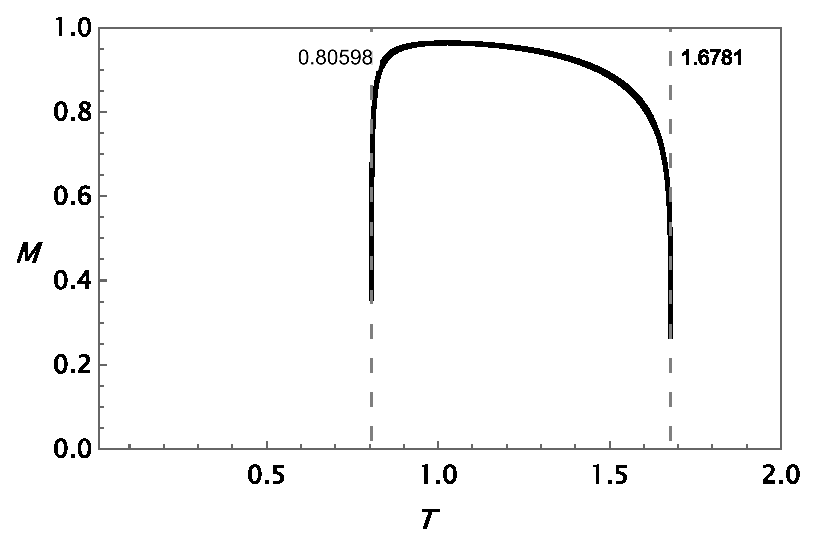
\includegraphics[width=1\linewidth]{part6/2transMag.eps} \\ б)}
	\end{minipage}
	\caption{$J_1 = 0.1, J_2 = -1.3, J_3 = -1.3, J_4 = -1.3, J_{d_1} = 1, J_{d_2} = 1, J_{d_3} = 1, J_{d_4} = 1$ и $d_1 = 4, d_2 = 4, d_3 = 4, d_4 = 4$}
	\label{2trans}
\end{figure}

 \begin{figure}[h]
	\begin{minipage}{0.47\linewidth}
		\center{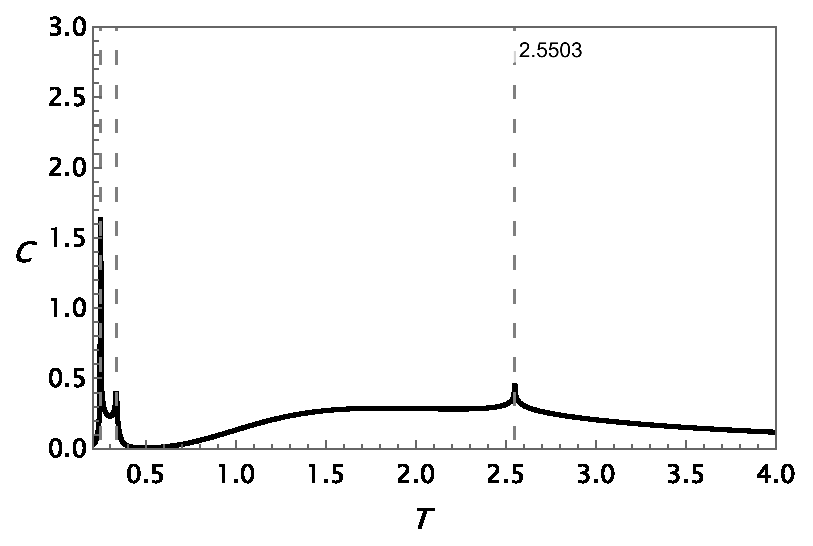
\includegraphics[width=1\linewidth]{part6/3transCapAll.eps} \\ а)}
	\end{minipage}
	\hfill
	\begin{minipage}{0.47\linewidth}
		\center{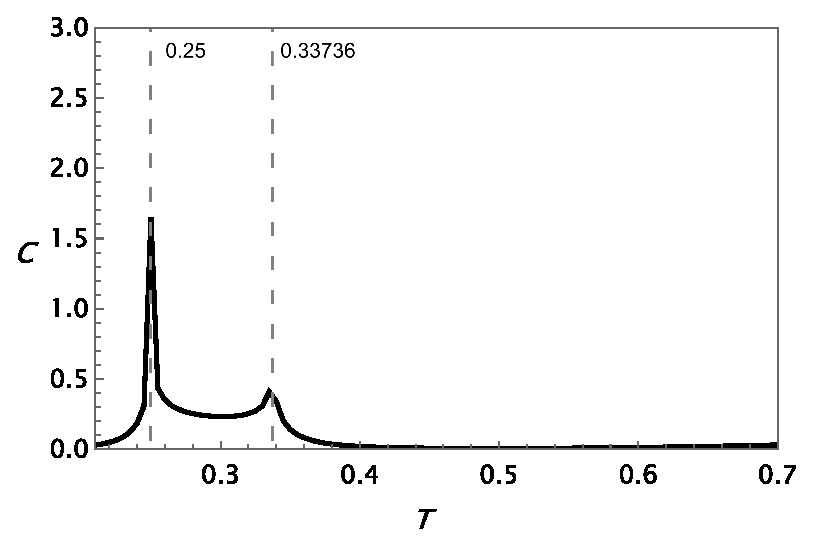
\includegraphics[width=1\linewidth]{part6/3transCapPart.eps} \\ б)}
	\end{minipage}
	\vfill
	\begin{minipage}{0.47\linewidth}
		\center{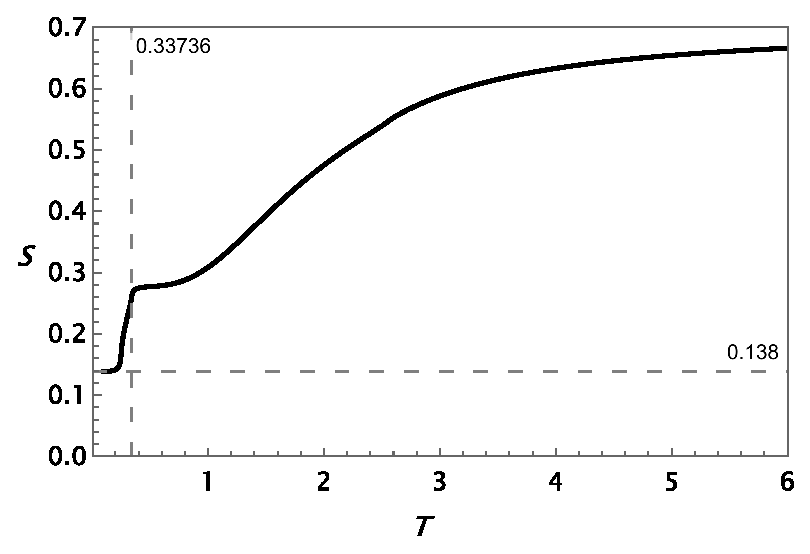
\includegraphics[width=1\linewidth]{part6/3transEnt.eps} \\ а)}
	\end{minipage}
	\hfill
	\begin{minipage}{0.47\linewidth}
		\center{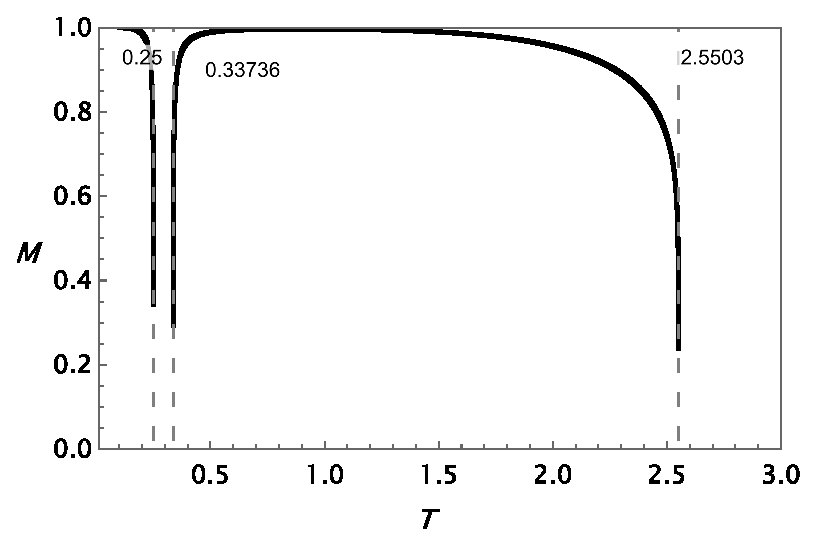
\includegraphics[width=1\linewidth]{part6/3transMag.eps} \\ б)}
	\end{minipage}
	\caption{$J_1 = -1.27, J_2 = -1, J_3 = -1.27, J_4 = -1, J_{d_1} = 1.3, J_{d_2} = 1.3, J_{d_3} = 1.3, J_{d_4} = 1.3$ и $d_1 = 7, d_2 = 7, d_3 = 7, d_4 = 7$}
	\label{3trans}
\end{figure}


 \begin{figure}[h]
	\begin{minipage}{0.47\linewidth}
		\center{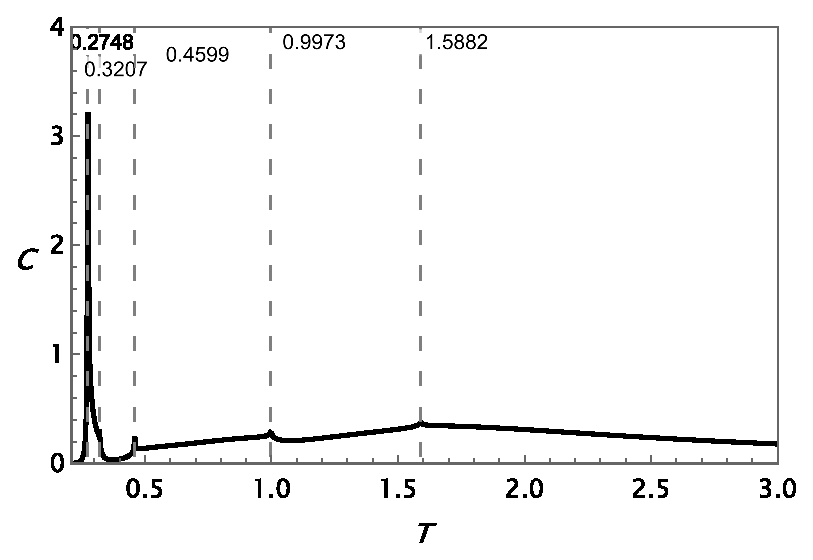
\includegraphics[width=1\linewidth]{part6/5transCapAll.eps} \\ а)}
	\end{minipage}
	\hfill
	\begin{minipage}{0.47\linewidth}
		\center{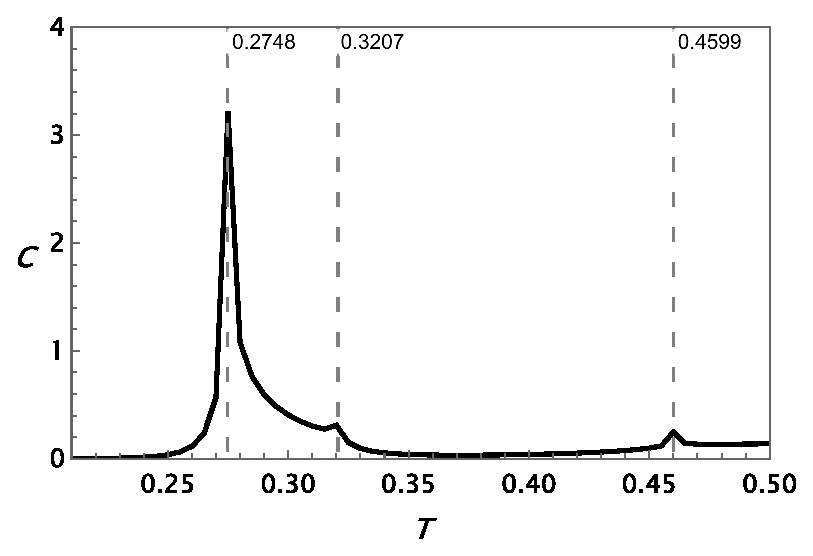
\includegraphics[width=1\linewidth]{part6/5transCapPart.eps} \\ б)}
	\end{minipage}
		\vfill
	\begin{minipage}{0.47\linewidth}
		\center{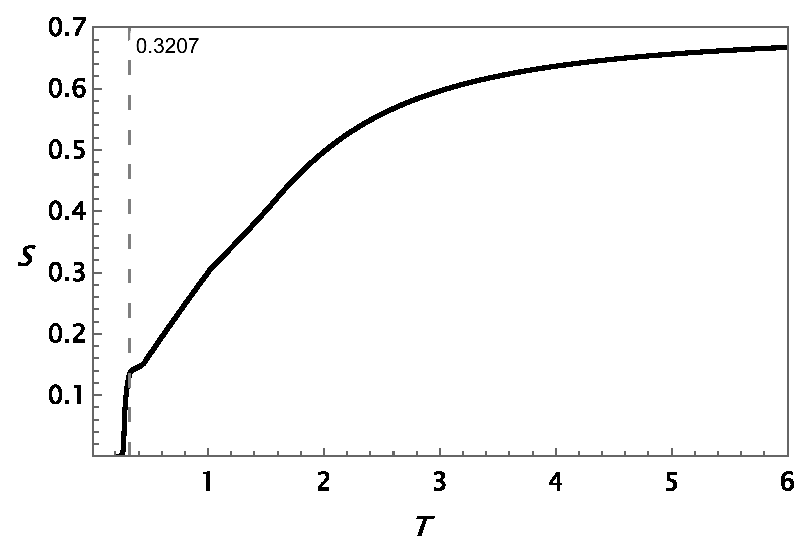
\includegraphics[width=1\linewidth]{part6/5transEnt.eps} \\ а)}
	\end{minipage}
	\hfill
	\begin{minipage}{0.47\linewidth}
		\center{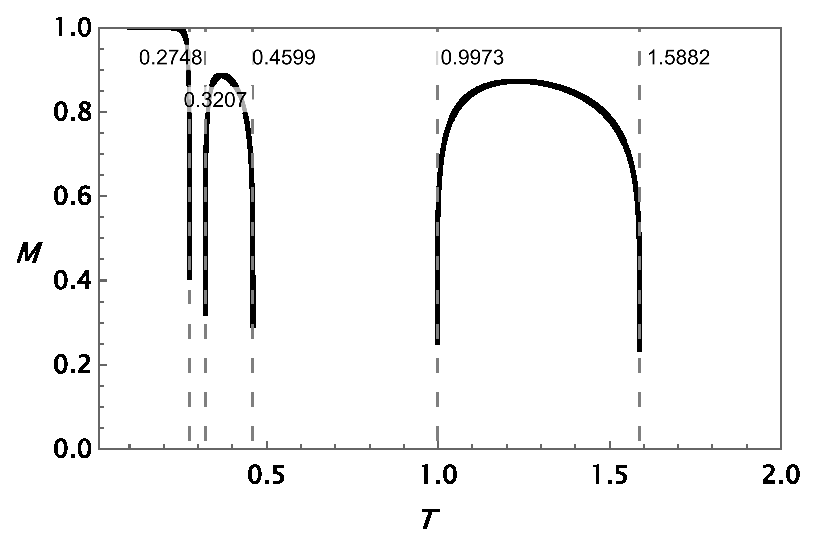
\includegraphics[width=1\linewidth]{part6/5transMag.eps} \\ б)}
	\end{minipage}
	\caption{$J_1 = -0.48621, J_2 = -1, J_3 = -0.671, J_4 = -1, J_{d_1} = 1.3, J_{d_2} = 1.3, J_{d_3} = 1.3, J_{d_4} = 1.3$ и $d_1 = 7, d_2 = 7, d_3 = 7, d_4 = 7$}
	\label{5trans}
\end{figure}

\section{Выводы по главе}

Выведено точное выражение для свободной энергии обобщенной модели Изинга с двумя трансляциями с учетом декорирования.

Выведено точное выражение для спонтанной намагниченности обобщенной модели Изинга с двумя трансляциями с учетом декорирования.

Исследованы термодинамические и фрустрационные свойства обобщенной модели Изинга с двумя трансляциями с учетом декорирования.

\FloatBarrier